\begin{figure}
    \centering
    \begin{subfigure}{0.48\linewidth}
        \centering
        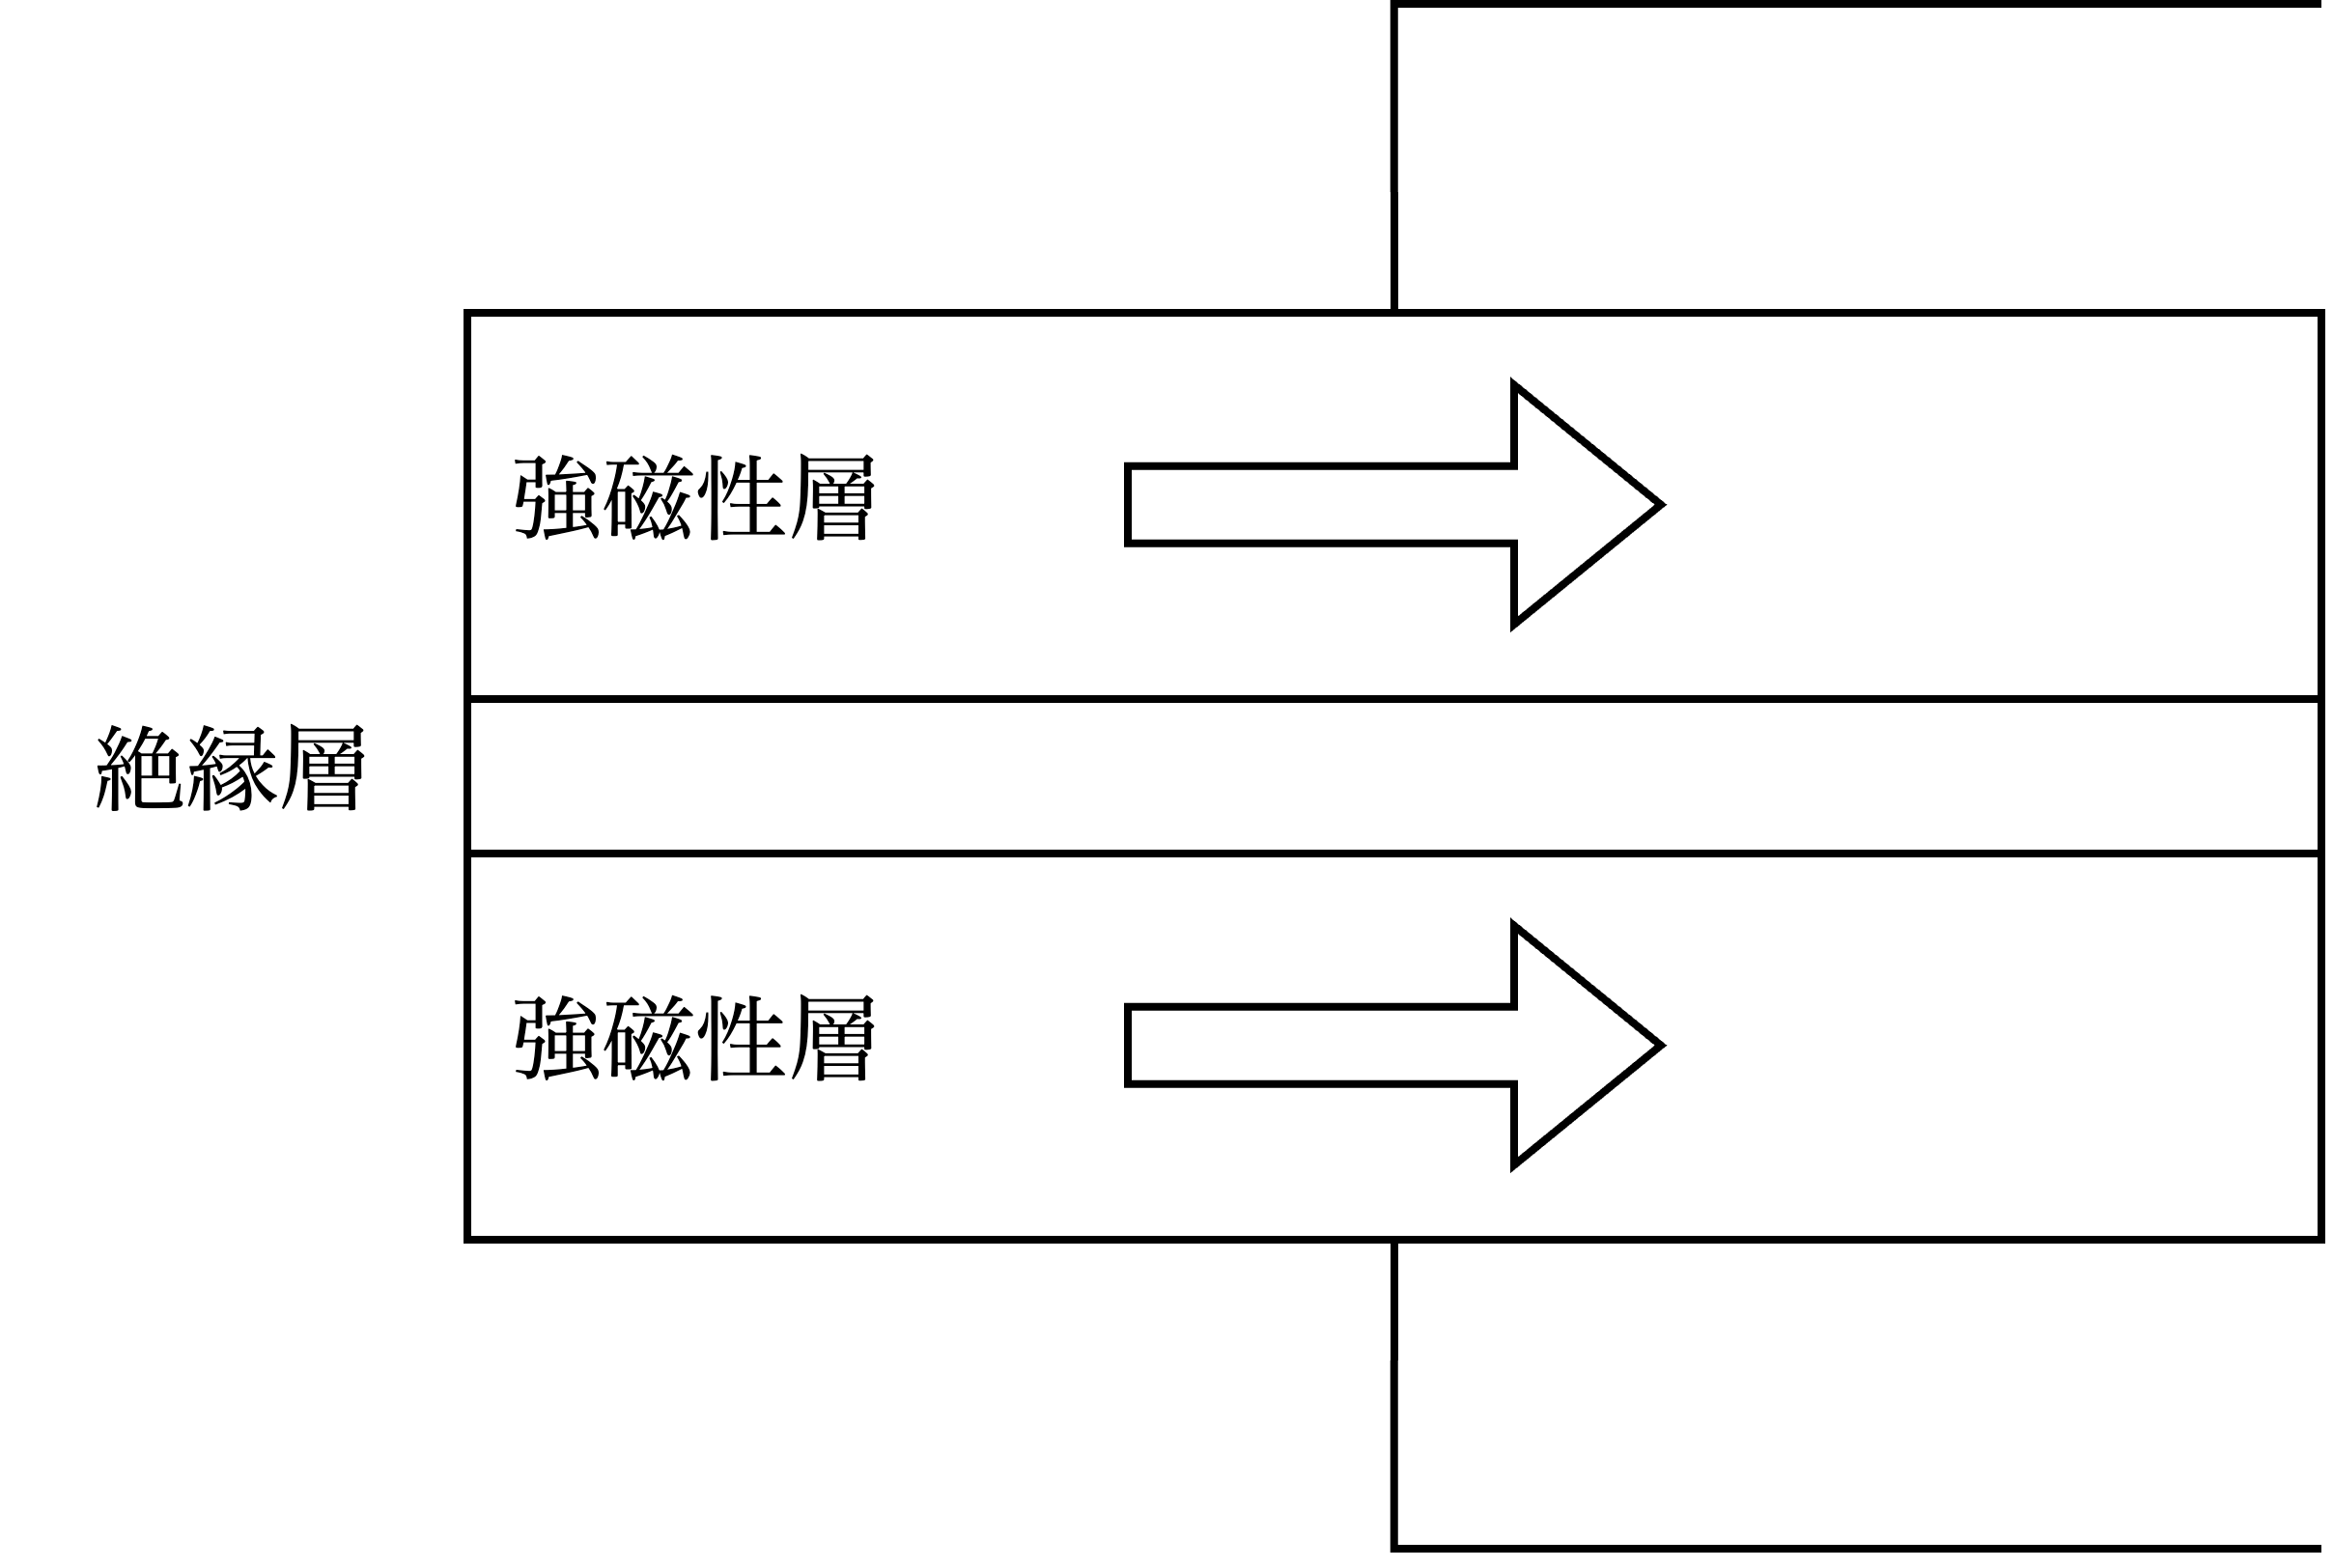
\includegraphics[width=0.8\linewidth]{src/figures/pri-tmr/tmr-p.png}
        \subcaption{磁化が平行の場合}\label{subfig:tmr-p}
    \end{subfigure}
    \begin{subfigure}{0.48\linewidth}
        \centering
        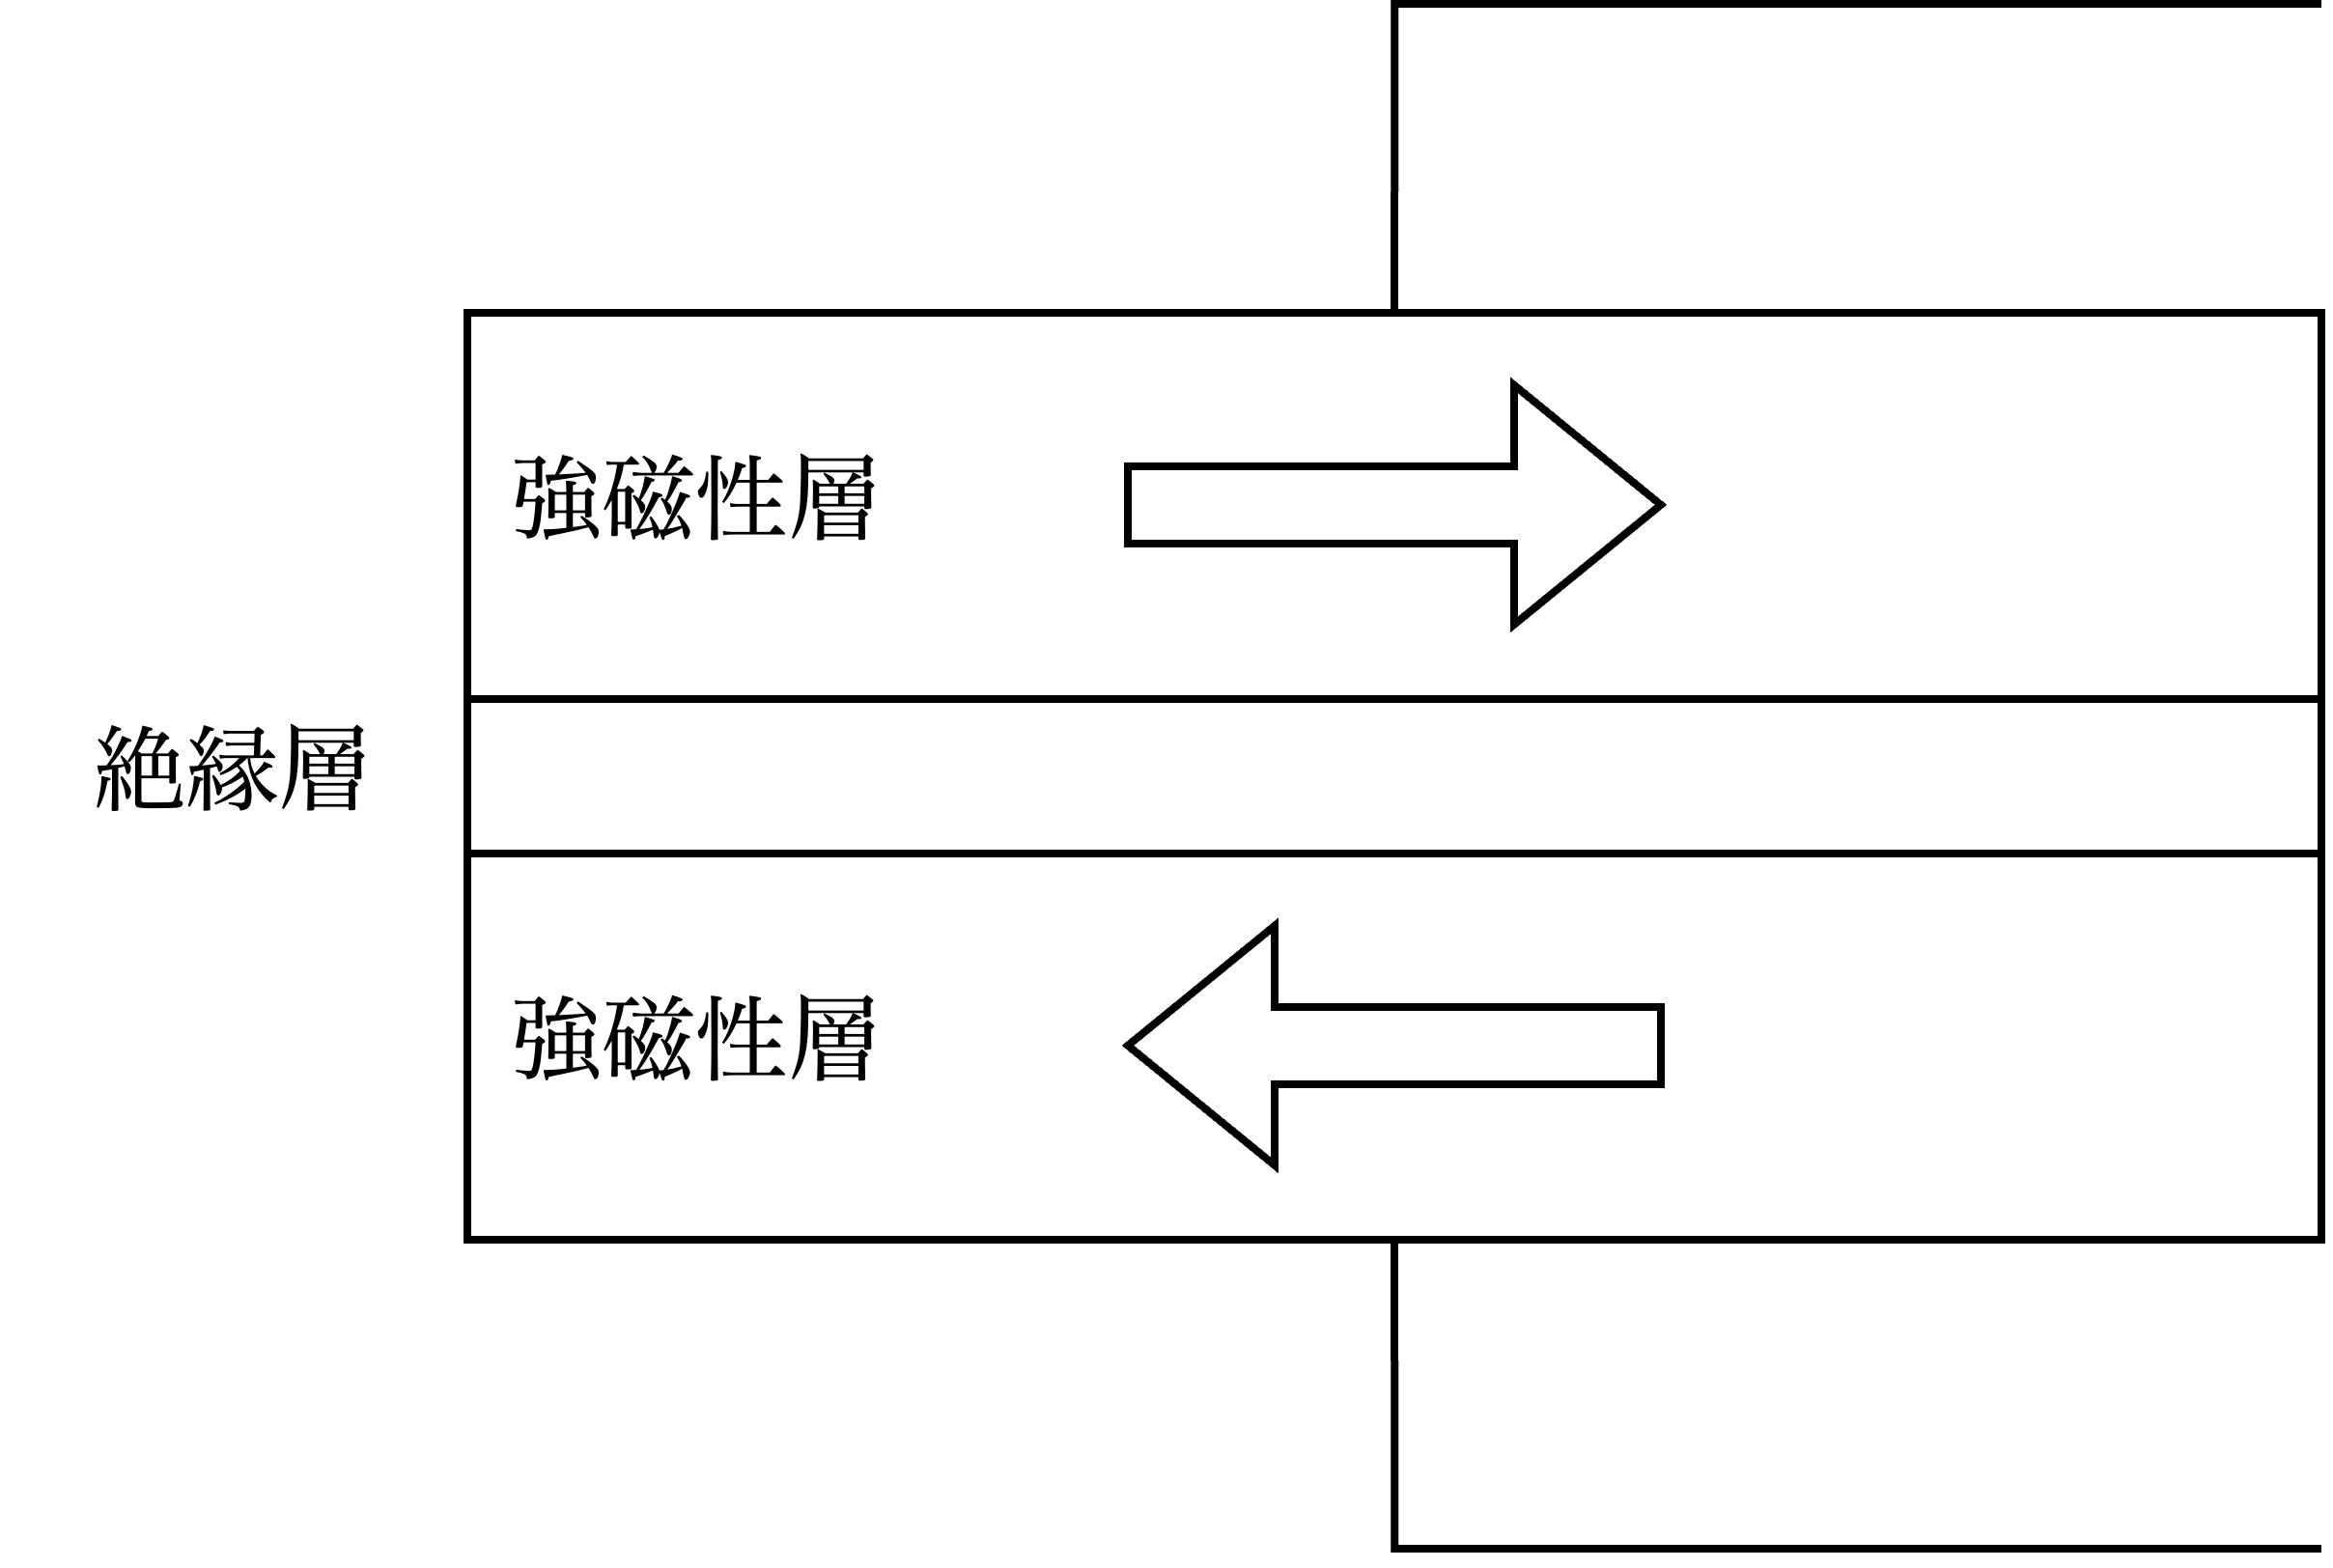
\includegraphics[width=0.8\linewidth]{src/figures/pri-tmr/tmr-ap.png}
        \subcaption{磁化が反平行の場合}\label{subfig:tmr-ap}
    \end{subfigure}
    \caption{MTJ(Magnetic Tunnel Junction)におけるTMR(Tunnel Magnetoresistance)効果}\label{fig:pri-tmr}
\end{figure}
